\section{Hardware Configuration}

All systems will be configured and connected to the same isolated network
through the hub as shown in Figure \ref{physical-setup}.

\begin{figure}[H]
  \centering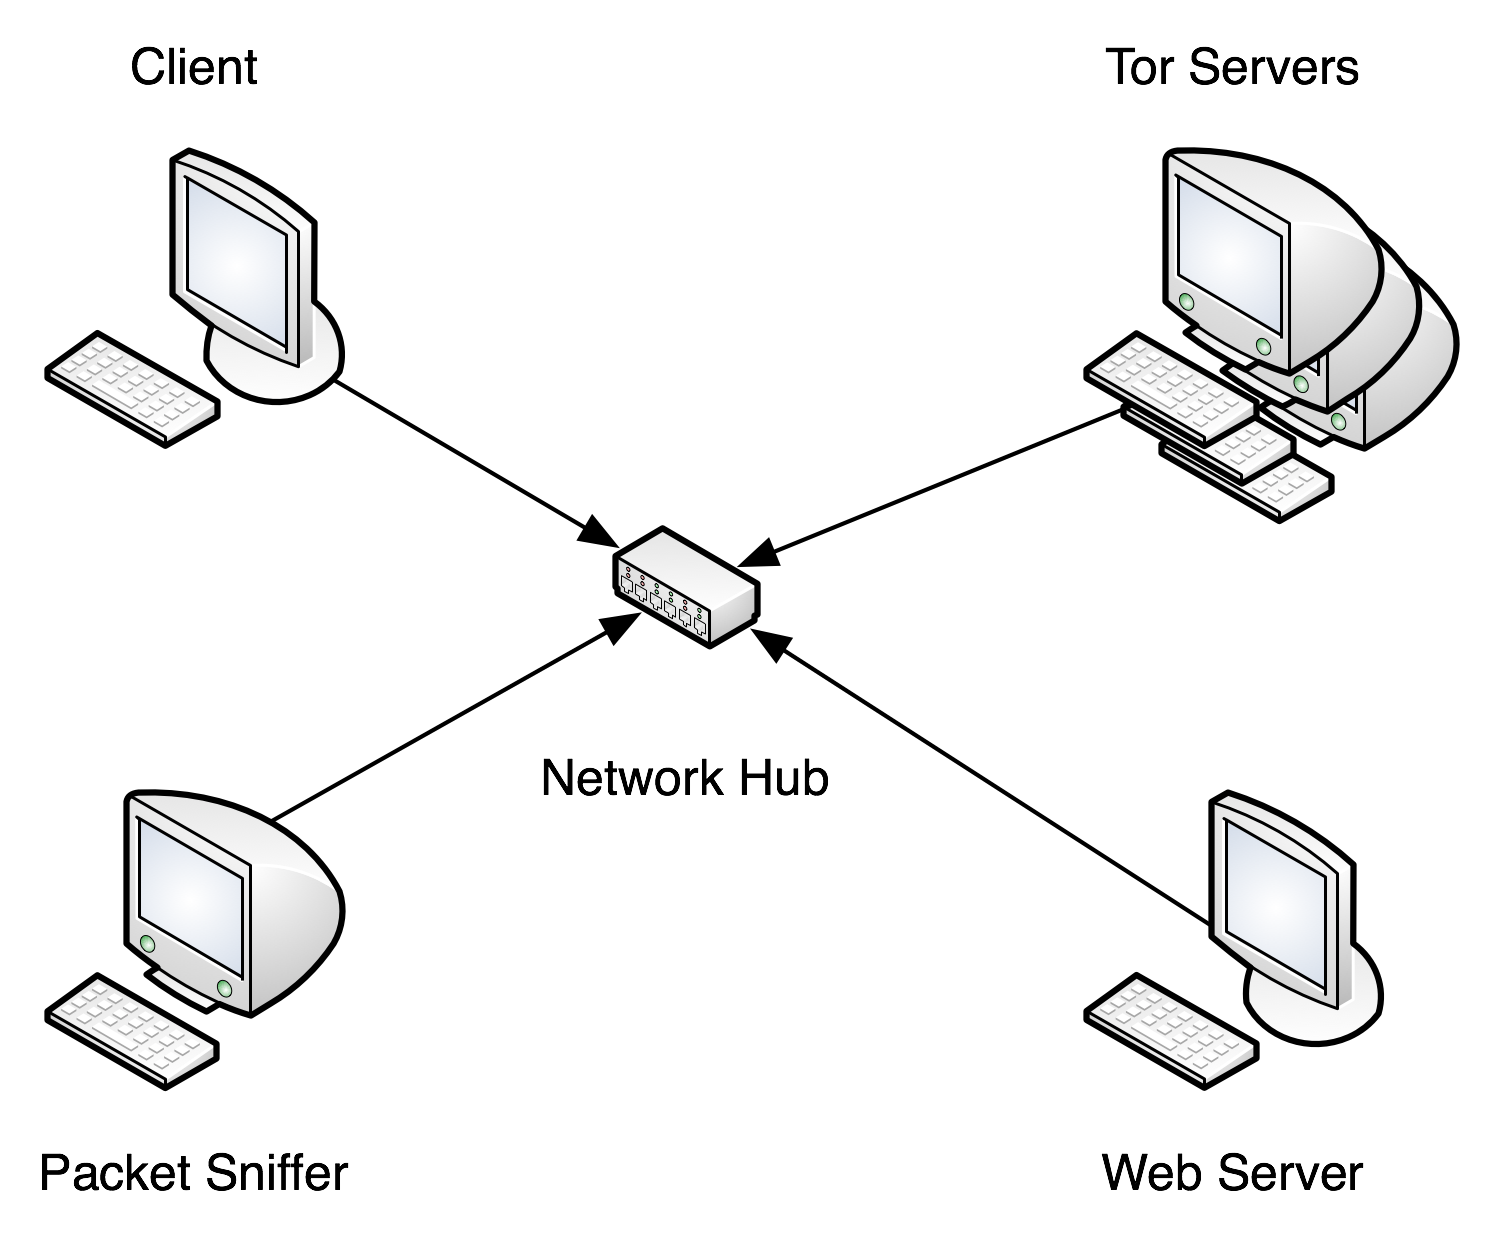
\includegraphics[scale=0.6]{physical-setup}
  \caption{Physical Setup}
  \label{physical-setup}
\end{figure}

\section{Software Configuration}

Software is installed and configured on all machines. The simulation network is
configured to use the private Tor directory server rather than the public ones
specified by default \parencite{website:private-tor-network}.

The packet sniffer is configured to capture only the packets relevant for each
data set.

Figure \ref{network-diagram} shows the placement of applications and relevant
data flows.

\begin{figure}[H]
  \centering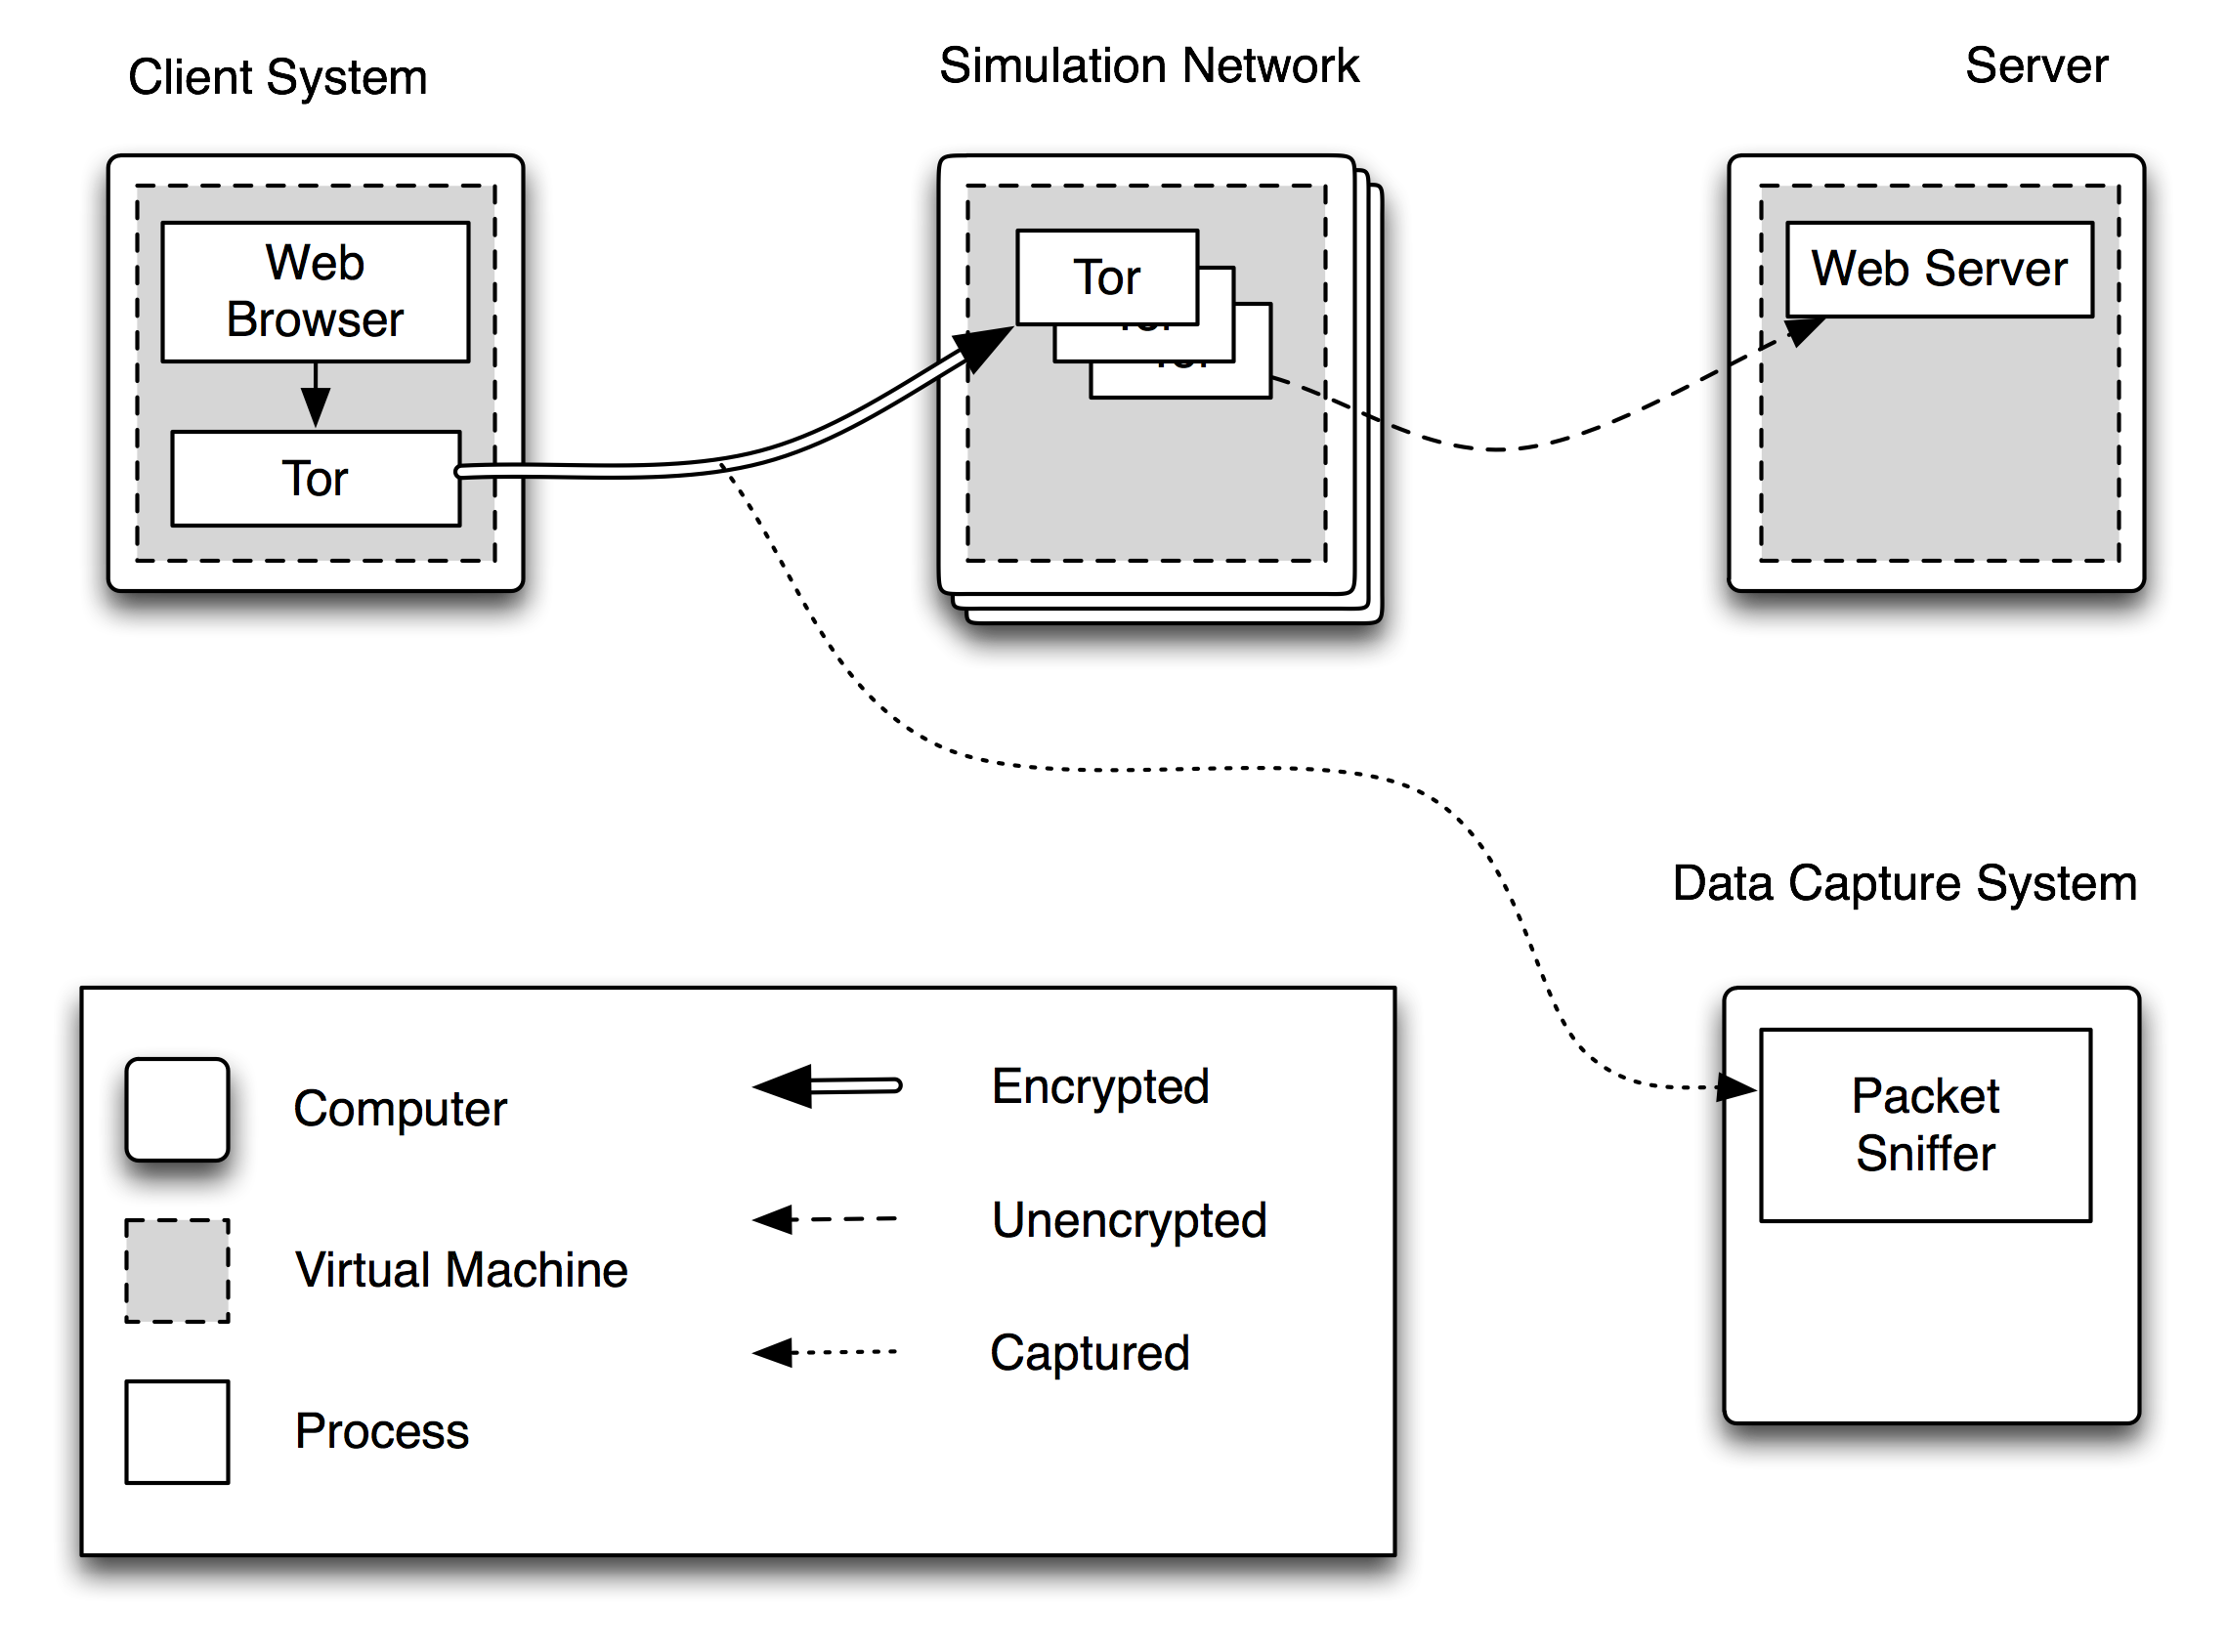
\includegraphics[width=\linewidth]{network-diagram}
  \caption{Network Diagram}
  \label{network-diagram}
\end{figure}

\section{Systems}

A number of systems will be configured both physical and virtual. The \emph{Host Systems}, those running natively on a physical PC with a Virtual Box environment to host a Guest Operating System. The \emph{Guest Systems}, operating systems running inside a Virtual Box environment on top of a Host System, and the Sniffing system, which is responsible for capturing the experiment results.

The name, IP Address and role of each system in the simulation network is shown in Table \ref{table:hosts}.

\begin{tabular}{lrr}
  \toprule
  Host Name & IP Address & Role\\
  \midrule
  Grumman & 192.168.0.100 & Management and Host of Client System \\
  Arrakis & 192.168.0.001 & Host of Server System \\
  Richese & 192.168.0.102 & Host of Tor Network System \\
  \midrule
  Ipyr & 192.168.0.200 & Sniffing System \\
  \midrule
  Lankiveil & 192.168.0.16 & Client Guest System \\
  Ginaz & 192.168.0.17 & Server Guest System \\
  Sikun & 192.168.0.18 & Tor Network Guest System \\
  \botomrule
  \label{table:hosts}
\end{tabular}

\subsection{Sniffing System}

The sniffing system has a very basic role: to capture packets. It is configured with the Ubuntu 10.04 Server Operating system. Most basic features are disabled and tcpdump is configured to run at startup saving all captures to 1mb files in a directory indicating when the system was booted.

\subsection{Host Systems}

All the host systems are configured identically. The following procedure is carried out to prepare a host system.

\begin{itemize*}
  \item Install Ubuntu 10.04 Desktop Operating System
    \begin{itemize*}
      \item Use entire disk
      \item Set time zone to GMT +8 WST (Perth)
    \end{itemize*}
  \item Turn off automatic package updates
  \item Turn off powersaving features
  \item Install OpenSSH Server
  \item Add Virtual Box repository to sources.lst
  \item Update sources and install Virtual Box
  \item Ensure Virtual Box starts with system and disable all other startup applications
\end{itemize*}

One of the host systems is set aside as a management system, which is responsible for ensuring the experiment runs and restarts it if there are any problems. On this machine a private ssh key is created, and copied to the authorized keys file on all other hosts. This allows the management system to connect to all the other systems and issue commands without user interaction.

The management script runs on the management system to watch the experiment's progress. This is a simple Ruby script which uses SSH to control the other Host systems and opens a socket which waits for a connection that indicates that the experiment has finished. Every time it starts the experiment, it rolls back each virtual machine to a preconfigured snapshot. If the experiment takes too long, say because a virtual machine hangs or something is wrong, it will be started without waiting for the finish condition.

Note that restarting each snapshot ensures that the system clock of each guest operating system is synchronized with that of the host operating system. The Tor network is sensitive to differences in time between hosts and this ensures correct operation.

\subsection{Guest Systems}

\subsubsection{Client System}

The client system runs Ubuntu 10.04 Desktop Operating System as well as a number of applications that allow it to perform automated web browsing. Tor is configured on this system as well for the Tor part of the experiment but is initially disabled.

The software installed on this system includes:

\begin{itemize*}
  \item Ruby
  \item Rubygems:
    \begin{itemize*}
      \item Selenium
      \item DaemonController
      \item RSpec
    \end{itemize*}
  \item Selenium-RC
  \item Firefox web browser
  \item Tor
\end{itemize*}

The client operation is controlled by a Ruby script which ensures that the Selenium-RC server is running, executes a number of Selenium browser simulations using RSpec and reports it's success by connecting to an open socket on the management system.

There are 170 simulations which emulate simple website interactions which have different traffic profiles against 30 different websites on the Server system.

For the non-SSL portion of the experiment, Selenium is configured to use a special proxy which automatically accepts self signed certificates. Typical interactions with SSL encrypted websites are signed by a certificate authority, so no user interaction is required to begin browsing.

\subsubsection{Server System}

The host system runs an apache web server which serves two sets of sample websites, static and dynamic. The static websites are served each from a different numbered directory and accessible over a different virtual host. This means that when a web browser is pointed at the directory \verb+site1.static.torsim+ the files in \verb+/var/www/thesis/experiment/simulation/static/site1+ are served to the browser.

For the SSL part of the experiment, only the HTTPS port 443 is accessed and all information is sent to the browser using encryption.

The dynamic sample websites change subtly with each attempted access. There are 10 sample websites each a slightly different Ruby Sinatra application.

\subsubsection{Tor Simulation}

The Tor Simulation Guest is responsible for emulating a Tor network. It runs three Tor directory authorities as well as fifteen relays.

Each Tor instance on the Tor Simulation system is given it's own separate directory for configuration, logging and temporary files.

\section{Procedure}

\subsection{Preparation}

\subsubsection{Host Systems}

The preparation for the host operating systems is identical except for the hostname and IP address.

Installing the Host operating system:

\begin{enumerate*}
  \item Power on machine
  \item Interrupt BIOS boot process
  \begin{enumerate*}
    \item Load default BIOS settings
    \item Set boot order to ensure CD-ROM is first
    \item Disable unnecessary boot devices
    \item Ensure system clock is correct
  \end{enumerate*}
  \item Boot from Ubuntu 10.04 Desktop cd
  \item Select the language you wish to use for installation (English) and click 'Forward'
  \item Select the region (Australia/Perth) and click 'Forward'
  \item Select an appropriate keymap (USA) and click 'Forward'
  \item Select 'Erase and use the entire disk' and click 'Forward'
  \item Enter your details, select 'Log in automatically' and click 'Forward'
\end{enumerate*}

At this point the installation will begin and should take about 35 minutes. 'Log in automatically' is selected to ensure that the experiment will continue even if power is lost. Once installation is complete remove the CD and reboot the system.

Configuring the Host operating system:

\begin{enumerate*}
  \item Configure the network adapter
  \item Install Virtual Box
  \item Load the guest operating system virtual machine image
\end{enumerate*}

To install Virtual Box, the following procedure is used:

\begin{enumerate*}
  \item Edit the file \verb+/etc/apt/sources.lst+ and add the line:
  \begin{verbatim}
deb http://download.virtualbox.org/virtualbox/debian lucid non-free
  \end{verbatim}
  \item Install the GPG key for the Virtual Box packages:
  \begin{verbatim}
wget -q http://download.virtualbox.org/virtualbox/debian/oracle_vbox.asc -O- | sudo apt-key add -
  \end{verbatim}
  \item Then install VirtualBox 3.2 with the command:
  \begin{verbatim}
sudo apt-get update && sudo apt-get install virtualbox-3.2
  \end{verbatim}
\end{enumerate*}

For the management system, some additional commands need to be run:

\begin{enumerate*}
  \item Generate a private ssh key for the user with the command: \verb+ssh-keygen+, when prompted for a password enter nothing.
  \item SSH to the other host systems on the network, and copy the contents of \verb+$HOME/.ssh/id_rsa.pub+ into \verb+$HOME/.ssh/authorized_keys+ on the destination system.
  \item Install ruby so that the management script can be run:
    \begin{verbatim}
sudo apt-get install ruby rubygems
    \end{verbatim}
  \item Ensure the script \verb+run_simulation.rb+ is started on login.
\end{enumerate*}

\subsubsection{Tor System}

Install Ubuntu 10.04 Server.

Deploy the experiment files.

Install Tor:

\begin{enumerate*}
  \item Edit the file \verb+/etc/apt/sources.lst+ and add the line:
  \begin{verbatim}
deb http://deb.torproject.org/torproject.org lucid main
  \end{verbatim}
  \item Install the GPG key for the Tor packages:
  \begin{verbatim}
gpg --keyserver keys.gnupg.net --recv 886DDD89
gpg --export A3C4F0F979CAA22CDBA8F512EE8CBC9E886DDD89 | sudo apt-key add -
  \end{verbatim}
  \item Install Tor:
  \begin{verbatim}
sudo apt-get update && sudo apt-get install tor
  \end{verbatim}
\end{enumerate*}

\subsubsection{Client System}

Install Ubuntu 10.04 Desktop as in the Host system directions, leaving out the Virtual Box installation.

\begin{enumerate*}
  \item Deploy the experiment files onto the client system.
  \item Install Ruby
  \item Install the bundler ruby gem with the command:
    \begin{verbatim}
gem install bundler
    \end{verbatim}
  \item Install the required client ruby gems by executing the bundler from the client directory in the deployed experiment files.
    \begin{verbatim}
bundle install
    \end{verbatim}
  \item Ensure that the client script is executed at system startup.
\end{enumerate*}

\subsubsection{Configuring the Management Script}

Once all systems are deployed, the management script needs to be altered to

\subsection{Execution}

Running the experiment is a matter of ensuring all Host systems are powered on, if everything is configured correctly the experiment will continue to run until stopped manually.
